\documentclass[12pt, letterpaper]{article}
%\documentclass[12pt, letterpaper]{amsart}

%%%%%%%%%%%% LANGUAGE & ENCODING %%%%%%%%%%%%%%%%%
\usepackage[english]{babel}
\usepackage[utf8]{inputenc}%%%% to process umlauts and accents directly
%\usepackage{indentfirst}
%\usepackage{ucs}

%%%%%%%%%%% PACKAGES %%%%%%%%%%%%%%%%%%%%%%%%%%%%%
% For Hyperlinks
\usepackage[colorlinks,linkcolor=cyan,citecolor=magenta]{hyperref}

% Common math packages
\usepackage{amsthm, amsmath, amsfonts, amssymb, esint, mathrsfs, mathtools}
\usepackage{tensor} % To handle multi-index notation
\usepackage[capitalize,nameinlink]{cleveref} % Nice references
\crefname{equation}{}{} % Removes Eq. from equation references
\numberwithin{equation}{section} % Number equations within each section separately

% Extra symbols
\usepackage{stmaryrd} % contains \owedge  for Kulkarni-Nomizu product and some other special characters
\usepackage{commath} % contains \norm \abs

% Some useful packages
\usepackage{verbatim} %%% enables \begin{comment}    \end{comment}
\usepackage{enumerate} % allows different types of indices
\usepackage{float} % Handling figures

%%%%%%%%%%% MARGINS %%%%%%%%%%%%%%%%%%%%%%%%%%%%%%%%
% Margins
\usepackage[top=1in, bottom=1in, left=1in, right=1in]{geometry}

%%%%%%%%%%% CUSTOM NOTATION  %%%%%%%%%%%%%%%%%%%%%%
\newcommand{\N}{\mathbb{N}}
\newcommand{\Z}{\mathbb{Z}}
\newcommand{\Q}{\mathbb{Q}}
\newcommand{\R}{\mathbb{R}}
\newcommand{\C}{\mathbb{C}}
\newcommand{\K}{\mathbb{K}}

\newcommand{\f}{\mathfrak}
\newcommand{\ul}{\underline}
\newcommand{\mb}{\mathbb}
\newcommand{\mr}{\mathrm}
\newcommand{\mf}{\mathbf}
\newcommand{\mc}{\mathcal}
\newcommand{\e}{\emph}
\newcommand{\vp}{\varphi}
\newcommand{\ve}{\varepsilon}

\newcommand{\vol}{\operatorname{Vol}}
\newcommand{\diam}{\operatorname{diam}}
\newcommand{\dist}{\operatorname{dist}}
\newcommand{\dv}{\operatorname{div}}
\newcommand{\tr}{\operatorname{tr}}

\newcommand{\dd}{\; \mathrm{d}} %%%% d for integration dx
\newcommand{\wt}{\widetilde}
\newcommand{\ol}{\overline}

%%%%%%%%%%% THEOREMS %%%%%%%%%%%%%%%%%%%%%%%%
\newtheorem{theorem}{Theorem}[section]
\newtheorem{lemma}[theorem]{Lemma}
\newtheorem{proposition}[theorem]{Proposition}
\newtheorem{conjecture}[theorem]{Conjecture}
\newtheorem{corollary}[theorem]{Corollary}
\newtheorem{claim}[theorem]{Claim}
\newtheorem{problem}[theorem]{Problem}
\newtheorem{remark}[theorem]{Remark}

\theoremstyle{definition}
\newtheorem{definition}[theorem]{Definition}

\theoremstyle{remark}
\newtheorem{example}[theorem]{Example}


%%%%%%%%%%% TITLE %%%%%%%%%%%%%%%%%%%
%\title[CIS625: Computational Learning Theory]{Computational Learning Theory Lecture Notes}
%\author[Notes by Martin Citoler-Saumell]{Martin Citoler-Saumell}
%\date{Spring 2017}
%\address{University of Pennsylvania\\ Philadelphia, PA 19104}
%\email{\href{mailto:martinci@math.upenn.edu}{martinci@math.upenn.edu}}

\title{Computational Learning Theory Lecture Notes}
\author{Martin Citoler-Saumell}
\date{CIS625 Spring 2017}

%%%%%%%%%%% DOCUMENT BEGINS %%%%%%%%%%%%
\begin{document}
%------------------------------------------------------------
%          LECTURE 4
%------------------------------------------------------------
\section{Lecture 4: 2017.02.13}

\begin{example}[Hyperplanes in $\R^2$]
    It is clear that the VCD is at least 3 because given three points, we can always choose a line that separates the points in any way we want. In fact, the VCD is exactly 3.
    \begin{figure}[H]
    \centering
    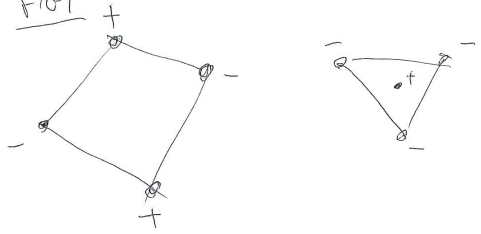
\includegraphics[width=0.3\linewidth]{img/hyperplanes.png}
    \end{figure}
    In general, for hyperplanes in $\R^d$ the VCD dimension is $d+1$.
\end{example}

\begin{example}[Convex n-gons in $\R^2$]
    In this case, $VCD = 2n+1$. For example, if $n=4$, $VCD = 9$.
    \begin{figure}[H]
    \centering
    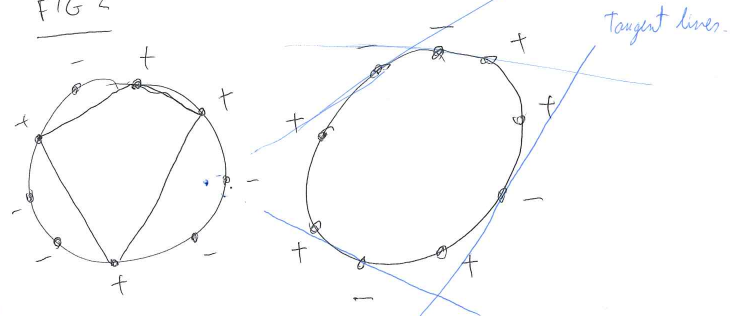
\includegraphics[width=0.3\linewidth]{img/4-gons.png}
    \end{figure}
\end{example}

\begin{remark}
    Note that in these geometric situations, the VCD dimension is linearly related to the free parameters in our model. This is generally true (more or less). This supports the idea that we need more samples than parameters to be able to start learning something significant.
\end{remark}

\begin{remark}[Monotone conjunctions over $\lbrace 0,1 \rbrace^m$ e.g. $x_1\land x_5\land x_7$]
    We claim that $VCD \geq n$. Indeed, consider the bit vectors: $\langle01\ldots 1\rangle, \langle 101\ldots 1\rangle, \ldots, \langle1\ldots 10\rangle$. We can always find a conjunction with the desired label. Namely, $x_1\land\ldots \land x_i^\lor\land\ldots\land x_n$ or its negation as needed.
\end{remark}

\subsubsection*{Overloaded Notation}
\begin{align}
    \Pi_{\mc C}(m) &\coloneqq \max\limits_{S\;:\;\abs{S}= m}\left\{\abs{\Pi_{\mc C}(S)}\right\}\\
    &= \textrm{max. \# of labelings induced by $\mc C$ on m points.}
\end{align}
Note that we have the following:
\begin{itemize}
    \item  $\Pi_{\mc C}(m)\leq 2^m$.
    \item If $m\leq VCD(\mc C)$, $\Pi_{\mc C}(m)=2^m$. 
    \item If  $m > VCD(\mc C)$, $\Pi_{\mc C}(m) < 2^m$.
\end{itemize} 

\begin{theorem}\label{main thm lecture 4}
    Let $VCD(\mc C)=d$. Then $\Pi_{\mc C}(m) = O(m^d)$.
\end{theorem}

\begin{remark}
    As the sample size becomes large compared to the dimension, the growth rate of $\Pi_{\mc C}(m)$ is sub-exponential. In fact, the fraction of possible behaviors grows like $\frac{\frac1{m^d}}{2^m}$ which tends to 0 as $m\to\infty$.
\end{remark}

\subsubsection*{Proof of \cref{main thm lecture 4}}
Consider $\phi_d(m) \coloneqq \phi_d(m-1) + \phi_{d-1}(m-1)$ with boundary conditions $\phi_0(m)=\phi_d(0)=1$.  We first prove the following lemma.
\begin{lemma}
    If $VCD(\mc C)= d$, then for any m we have $\Pi_{\mc C}(m) \leq \phi_d(m)$.
\end{lemma}
\begin{proof}
   We use a double induction argument. The base cases are clear so assume the lemma is true for any $d'\leq d$ and $m'\leq m$ with at least one the inequalities being $<$. Consider the set $S=\lbrace x_1,\ldots,x_m\rbrace$. Recall that $\Pi_{\mc C}(S)$ is just the possible labelings of $S$ that can be realized with concepts in $\mc C$. Now consider all the possible labelings that are possible for $\lbrace x_1,\ldots,x_{m-1}\rbrace = S\setminus \lbrace x_m\rbrace$. For each of these, there are exactly 2 potential labelings for $S$ depending on whether $x_m = 0$ or $x_m = 1$. Then, by the induction hypothesis, we have
   \begin{align}
   \abs{\Pi_{\mc C}(S\setminus\{x_m\})} \leq \Pi_{\mc C}(m-1) \leq \phi_d(m-1).
   \end{align}
   Next consider the labelings of $S\setminus \lbrace x_m\rbrace$ that appear twice in the labelings of $S$. That is, those such that both $x_m = 0$ and $x_m = 1$ are possible labelings. Then we can shatter at most $d-1$ points with $S\setminus \lbrace x_m\rbrace$ because otherwise we would violate $VCD(\mc C) = d$. Finally, by induction hypothesis we have that
   \begin{align}
        \textrm{\# of labelings of $S\setminus \lbrace x_m\rbrace$ }\leq \phi_{d-1}(m-1).
   \end{align}
   Combining these two bound we obtain the result.
\end{proof}

\begin{claim}
    $\phi_d(m) = \sum\limits_{i=0}^d\binom{m}{i}$.
\end{claim}
\begin{proof}
    By induction,
    \begin{align}
        \phi_d(m) &= \phi_d(m-1) + \phi_{d-1}(m-1) = \sum\limits_{i=0}^d\binom{m-1}{i} + \sum\limits_{i=0}^{d-1}\binom{m-1}{i}\\
        &= \sum\limits_{i=0}^d\binom{m-1}{i} + \sum\limits_{i=0}^{d}\binom{m-1}{i-1}\\
        &= \sum\limits_{i=0}^d\left[\binom{m-1}{i} + \binom{m-1}{i}\right] = \sum\limits_{i=0}^d\binom{m}{i}.
    \end{align}
\end{proof}

Now the proof of \cref{main thm lecture 4} follows by noting that $\sum\limits_{i=0}^d\binom{m}{i} = O(m^d)$.

\subsection{Combinatorial $\rightarrow$ Probabilistic}
Fix target $c\in\mc C$ and a distribution $D$. Thinking of $c$ as a set, we can consider $\mc H\triangle c = \lbrace h\triangle c : h\in\mc H \rbrace$, which are the \emph{error regions}.
\begin{definition}
 We say that $S$ of m points is a \emph{$\ve$-net} for $\mc H\triangle c$ if for all $r\in\mc H\triangle c$ such that $D[r]\geq \ve$, then we have $S\cap r \ne \emptyset$.
\end{definition}
\begin{remark}
$VCD(\mc H\triangle c) = VCD(\mc H)$. This is because taking the symmetric difference corresponds to a XOR operation.
\end{remark}
Consider the auxiliary function on $S = \lbrace x_1,\ldots,x_m\rbrace$
\begin{align}
    A(S)&\coloneqq
    \begin{cases}
    1\quad\textrm{if $S$ is not an $\ve$-net for $\mc H\triangle c$}\\
    0\quad\textrm{else}
    \end{cases},\\
    B\left(S, S'\right)&\coloneqq
    \begin{cases}
    1\quad\textrm{if $\exists r \in \mc H\triangle c$ st. $D[r]\geq\ve$, $r\cap S=\emptyset$, $\abs{r\cap S'}\geq \frac{\ve m}2$}\\
    0\quad\textrm{else}
    \end{cases}.
\end{align}
\begin{remark}
    Event $B\left(S, S'\right)$ occurs if $\exists r \in \mc H\triangle c$ st. $r$ is ``hit'':
    \begin{itemize}
    \item $l \geq \frac{\ve m}2$ times in $S\cup S'$ but \emph{all} $l$ fall in $S'$.
    \end{itemize}
\end{remark}
\begin{align}
    \mb P_{S, S'}[B(S, S')] &= \mb P_{S, S'}[ B(S, S') \left|\right. A(S)] \cdot  \mb P_{S, S'}[A(S)]\\
    &\geq \frac12  \mb P_{S, S'}[A(S)],
\end{align}
where we used Chebyshev's inequality on the last line.

\paragraph{Draw $\langle S, S'\rangle$ of $2m$ points in 2 steps:}
\begin{enumerate}
\item Draw $2m$ points randomly from the distribution $D$. $x_1,\ldots, x_m, x_{m+1},\ldots, x_{2m}$
\begin{enumerate}[-]
\item \# possible labelings of the $2m$ points by $\mc H \triangle c$ fixed $\leq \phi_d(2m)$.
\end{enumerate}
\item Split the $2m$ points randomly into $S$ and $S'$.
\end{enumerate}

\begin{claim}
$\mb P_{permutation}[B\left(S, S'\right)] = \frac{\binom{m}{l}}{\binom{2m}{l}}\leq 2^{-l}$.
\end{claim}
\begin{proof}
    Simple exercise in combinatorics.
\end{proof}
Then we have that
\begin{align}
    \mb P[B\left(S, S'\right)] \leq \phi_d(2m)2^{-\frac{\ve m}2} \leq C_0 (2m)^d 2^{-\frac{\ve m}2} \leq e^{C_1[d\log(m)-\ve m]}.
\end{align}
We have just proven the following theorem.
\begin{theorem}
    As long as $m\geq C_2\left(\frac1\ve\log\left(\frac1\delta
    \right) + \frac{d}\ve\log\left(\frac1\ve\right)\right)$, where $VCD(\mc H) = d$, we have that with probability $\geq 1-\delta$, any \emph{consistent} $h\in\mc H$ has error $\leq \ve$ with respect to $c$ and $D$.
\end{theorem}
\end{document}
